\documentclass[12pt,a4paper,ngerman]{scrartcl}
\usepackage[ngerman]{babel}
\usepackage[utf8]{inputenc}
\usepackage{csquotes}
\usepackage{graphicx}

\author{Thomas Hilarius Meyer\\ \textsf{thomas.hilarius.meyer@gmail.com}}

\title{Die Gersheimer Schulimkerei-Beute (GSIB)}
\subtitle{Überlegungen zu Konzeption, Bau und Betriebsweise}

\begin{document}
	\maketitle

\begin{abstract}
	Die Gersheimer Schulimkerei-Beute (GSIB) ist eine Trogbeute für 24 Zander-Rähmchen.
	Sie eignet sich besonders für den pädagogischen Umgang mit Bienen, da alle Waben in einer
	Ebene liegen und somit direkt einsehbar und zugänglich sind; im Umgang mit ihr sind
	keine schweren Gewichte zu heben und die Arbeitshöhe bleibt konstant.
	Alle Verfahren der modernen Magazin-Imkerei lassen sich mit der GSIB durchführen und
	ein späterer Wechsel der Jungimker etwa zur Liebigbeute ist problemlos möglich.
\end{abstract}

\section{Gestaltungsprinzipien}

Die Zeit ist reif für einen neuen Bienenkasten!


\subsection{Vorüberlegungen / Anforderungen}

Was müsste ein Schulbienenkasten besser können als die Liebig-Beute?

\begin{enumerate}
\item keine Zargen abheben müssen
  \begin{itemize}
  \item Frage der Kraft
  \item psychologische Hemmschwelle
  \item Störung der Bienen
  \end{itemize}
\item alle Teile des Bienenstocks sind gleichzeitig sichtbar
\item Zandermaß, um später leichter auf Magazinbeuten umsteigen zu können (eine Beute, aus der man \enquote{herauswächst}...
\item Betriebsweise sehr nahe an der Magazinimkerei (imkern lernen)
\item geringer Preis (OSB-Platten mit 20mm Stärke)
\end{enumerate}

In Kauf genommene Nachteile sind weitgehend irrelevant für den speziellen Zweck der \enquote{pädagogischen} Bienenbeute:

\begin{itemize}
\item Unwirtschaftliches Arbeiten (\enquote{wabenweise} statt \enquote{zargenweise})
\item schwieriges Wandern wegen des hohen Gewichts
\end{itemize}


\subsection{Konkrete Designentscheidungen}

Folgende Konstruktionsentscheidungen sind für den Entwurf maßgeblich:

\begin{itemize}
\item Zander-Rähmchen als verbreitetstes Rähmchenmaß
\item gleiches Maß im Brut- und Honigraum
\item vertikales Königinnenabsperrgitter möglich
\item Möglichkeit einer vertikalen Bienenflucht
\item extrem leichter Zusammenbau aus wenigen, einfachen Teilen
\end{itemize}


\section{Bisherige Ansätze}

Welche Bienenkästen mit grundsätzlich ähnlicher Konstruktion (Waben auf einer Ebene) gibt es schon und warum sind diese nicht geeignet?

\begin{description}
\item[Hohenheimer Einfachbeute] ideales System für \enquote{erwachsene} Imker; doch Nachteil: schweres Heben, Scheu des Zargen-Abhebens...
\item[Golzbeute] komplizierter Aufbau, teuer, spezielles Wabenmaß, keine Bienenflucht.
\item[Mellifera Einraumbeute] spezielles Wabenmaß, kein Abspergitter und keine Bienenflucht möglich.
\item[Top-Bar-Hive] Umstieg auf Magazin-Imkerei sehr kompliziert.
\item[Bienenkiste] extrem unergonomisch; Stabilbau verhindert Wabenkontrolle.
\item[Alpentrogbeute (V. Weber)] komplizierter Aufbau, schwer zu bekommen, Honigräume werden aufgesetzt!
\end{description}


\section{Bau}

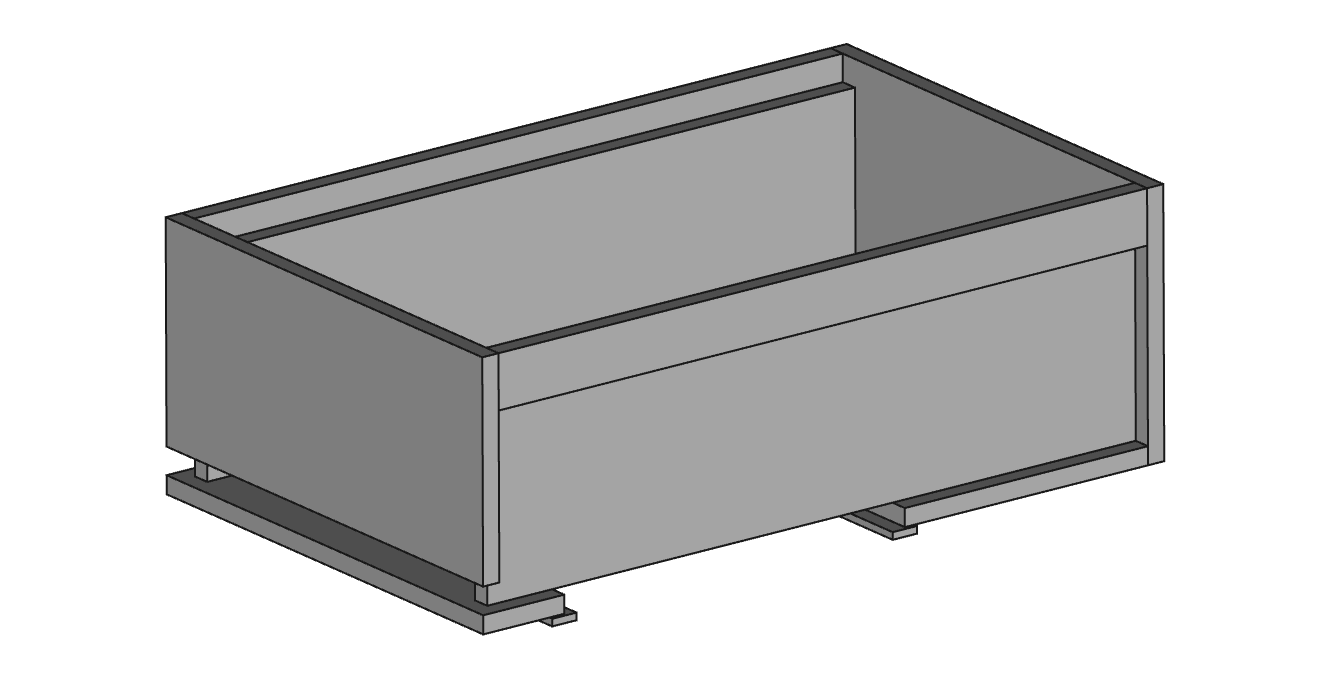
\includegraphics[width=\textwidth]{ansicht1}

[vgl. separate FreeCAD-Datei bzw. PDF-Pläne für konstruktive Details.]

\minisec{Teileliste}

\begin{center}
\begin{tabular}{lll}
  Bezeichnung &                       Maße [in mm] &          Anzahl \\
  \hline
  Seitenbrett links + rechts &        800 x 240 &             2 \\
  Seitl. Griffbrett links + rechts &  800 x 60 &              2 \\
  Stirnbrett vorne &                  520 x 240 &             1 \\
  Rückwand &                          520 x 290 &             1 \\
  Bodenbrett hinten &                 520 x 300 &             1 \\
  Bodenbrett vorne &                  520 x 100 &             1 \\
  Schubleisten &                      520 x 30 x 8 &          2 \\
  \hline
  Innendeckel (Dämmmaterial) &        840 x 520 &             1 \\
  \hline
\end{tabular}

[Materialstärke 20mm wenn nicht angegeben.]
\end{center}


\minisec{Zusatzteile}

\begin{itemize}
\item vertikales Königinnenabsperrgitter
\item vertikale Bienenflucht
\end{itemize}


\section{Offene Fragen}

\begin{enumerate}
%\item Boden: Öffnungen wegen Belüftung und besserer Varroabeobachtung? Oder reicht die Zugänglichkeit über das Flugloch?
%  (Stabilität der Konstruktion)
\item Notwendigkeit des Abspergitters: evtl. unnötig wg. des natürlichen Triebs der Königin, das Brutnest fluglochnah zusammenzuhalten?
\end{enumerate}


\section{Betriebsweise}

\subsection{Varroa: Winterbehandlung mit Oxalsäureverdampfer}

(Idee: Einblasloch im Fluglochstück? Entwicklung eines Verdampfers auf Basis eines Gasbrenners?)


\subsection{Ablegerbildung}

Entweder Bildung in der GSB (mit Fluglochverkleinerung und Volumenbegrenzungsschied)
oder in normalem Zander-Ablegerkasten


\subsection{Honigernte}

Benutzung des vertikalen Absperrgitters

vertikale Bienenflucht


\subsection{Varroa: Sommerbehandlung mit Ameisensäure}

Nassenheider Professional im bisherigen Honigraum


\subsection{Einfütterung}

Eimer im Honigraum


\section{Literaturhinweise}

\begin{enumerate}
\item Gerhard Liebig, Einfach imkern, (3. Aufl.) 2011.
\item Friedrich Pohl (Hg.), Bienenkiste, Korb und Einfachbeuten. Naturnah und erfolgreich imkern, Stuttgart 2013.
\item Vinzenz Weber, Leichter imkern mit Trogbeuten, München (2. Aufl.) 1990.
\end{enumerate}
\end{document}